\chapter{System Architecture and Design}

\section{System Architecture Overview}
Digital Mohalla is structured as an event-driven modular monolith. This architectural style was selected (ADR-0001) to eliminate distributed transaction complexities while preserving strict domain boundaries. The computational core (the Trust and Risk Assurance Engine) operates behind domain interfaces, decoupling mathematical inference from HTTP transport, database schemas, and client presentation frameworks.

\section{Architectural Style and Design Principles}
The platform adheres to Domain-Driven Design (DDD) and Clean Architecture principles:
\begin{itemize}
    \item \textbf{Single Source of Truth for State:} The borrowing transaction lifecycle is modeled as an append-only event stream. Current state is derived deterministically by replaying historical events through domain aggregates.
    \item \textbf{Separation of Assurance and Lifecycle:} Transaction states (\texttt{REQUEST\_CREATED}, \texttt{ACCEPTED}, \texttt{ACTIVE}, \texttt{COMPLETED}) represent real-world physical stages, whereas assurance evaluations (\texttt{SUFFICIENT\_EVIDENCE}, \texttt{SUFFICIENT\_WITH\_SAFEGUARDS}, \texttt{INSUFFICIENT\_EVIDENCE}) represent decision support. Assurance output advises lenders but never mutates lifecycle state automatically.
    \item \textbf{Database-Enforced Concurrency:} Invariants that must hold under concurrent client access (such as no-double-booking and append-only immutability) are enforced directly at the PostgreSQL storage boundary.
\end{itemize}

\section{System Layers and Subsystems}
\begin{enumerate}
    \item \textbf{Presentation Layer (React Native / Expo):} Cross-platform web and mobile interface. Implements responsive UI themes (Terracotta, Cream Green), the 3-layer lender evidence dashboard, and dual-party confirmation flows.
    \item \textbf{API Transport Layer (FastAPI):} Exposes RESTful endpoints under \texttt{/api/v1}. Validates incoming JSON payloads using Pydantic v2 schemas, handles JWT bearer authentication, and formats outgoing responses.
    \item \textbf{Application Service Layer (\texttt{BorrowingService}):} Coordinates domain commands, loads aggregates from the event store, executes locality boundary checks, invokes the assurance engine, and persists newly generated events.
    \item \textbf{Domain Core Layer:} Pure business logic containing the \texttt{BorrowingTransaction} aggregate, \texttt{TransitionTable}, Bayesian Beta estimators, bounded $k$-hop graph algorithms, and decision policy rules. Has zero dependencies on external databases or web frameworks.
    \item \textbf{Persistence Layer (SQLAlchemy \& PostgreSQL 16):} Manages the immutable event table (\texttt{lifecycle\_events}), read-model projections (\texttt{transactions}, \texttt{trust\_edges}), and database triggers.
\end{enumerate}

\section{Core Interfaces and Domain Contracts}
The system architecture defines five foundational domain interfaces:
\begin{table}[htbp]
\centering
\caption{Foundational Domain Interfaces and Contracts}
\label{tab:core_interfaces}
\small
\begin{tabularx}{\textwidth}{l p{5cm} p{7cm}}
\toprule
\textbf{Interface} & \textbf{Contract Method} & \textbf{Architectural Responsibility} \\
\midrule
\texttt{IBorrowingService} & \texttt{create\_request}, \texttt{accept}, \texttt{handover}, \texttt{return} & Coordinates lifecycle command execution and audit rejection logging. \\
\texttt{IAssess} & \texttt{assess(request) -> AssessmentResult} & Core assurance abstraction; decouples lifecycle from the Bayesian engine. \\
\texttt{IIndirectEvidence} & \texttt{find\_paths(src, dst, max\_k)} & Traverses community trust graphs to discover bounded indirect trust paths. \\
\texttt{IOutcomeSink} & \texttt{record\_outcome(event)} & Listens to closing lifecycle events and records verified interaction metrics. \\
\texttt{IEventStore} & \texttt{append}, \texttt{load\_stream}, \texttt{verify\_chain} & Manages append-only persistence, stream sequence checks, and hash chaining. \\
\bottomrule
\end{tabularx}
\end{table}

\section{Architectural Decision Records (ADR Summary)}
The project architecture is governed by formal Architectural Decision Records:
\begin{itemize}
    \item \textbf{ADR-0001 (Modular Monolith Architecture):} Selected over microservices to avoid distributed consensus latency, simplify local developer testing, and allow direct in-memory engine invocations.
    \item \textbf{ADR-0002 (Event Sourcing for Borrowing Transactions):} Mandates append-only event logs for all lifecycle state transitions, guaranteeing verifiable audit trails for dispute resolution.
    \item \textbf{ADR-0003 (PostgreSQL 16 Exclusion Constraints for Concurrency):} Uses \texttt{btree\_gist} exclusion constraints over item ID and date ranges (\texttt{tsrange}) to mathematically prevent overlapping accepted reservations.
    \item \textbf{ADR-0004 (Decoupled Assurance Boundary):} Encapsulates all trust mathematics behind the \texttt{IAssess} interface, enabling seamless replacement of stubs with full Bayesian estimators without altering lifecycle code.
    \item \textbf{ADR-0005 (Technology Stack Selection):} Standardizes on Python 3.12 (FastAPI), PostgreSQL 16, Expo (React Native with TypeScript), and GitHub Actions CI.
    \item \textbf{ADR-0006 (Trust-Edge Weighting Rule - Experimental):} Defines trust edge strength from verified outcomes as $\text{weight} = \frac{1 + s_w}{2 + s_w + f_w}$ with direct prior parameters and 180-day half-life decay.
    \item \textbf{ADR-0007 (Privacy-Preserving Locality):} Eliminates raw GPS coordinate storage, storing only coarse neighbourhood boundary membership tokens.
    \item \textbf{ADR-0008 (Bounded Indirect Evidence):} Restricts trust propagation to $k \le 3$ hops with path decay and an absolute support cap of 0.30 to prevent sybil domination.
\end{itemize}

\begin{figure}[htbp]
\centering
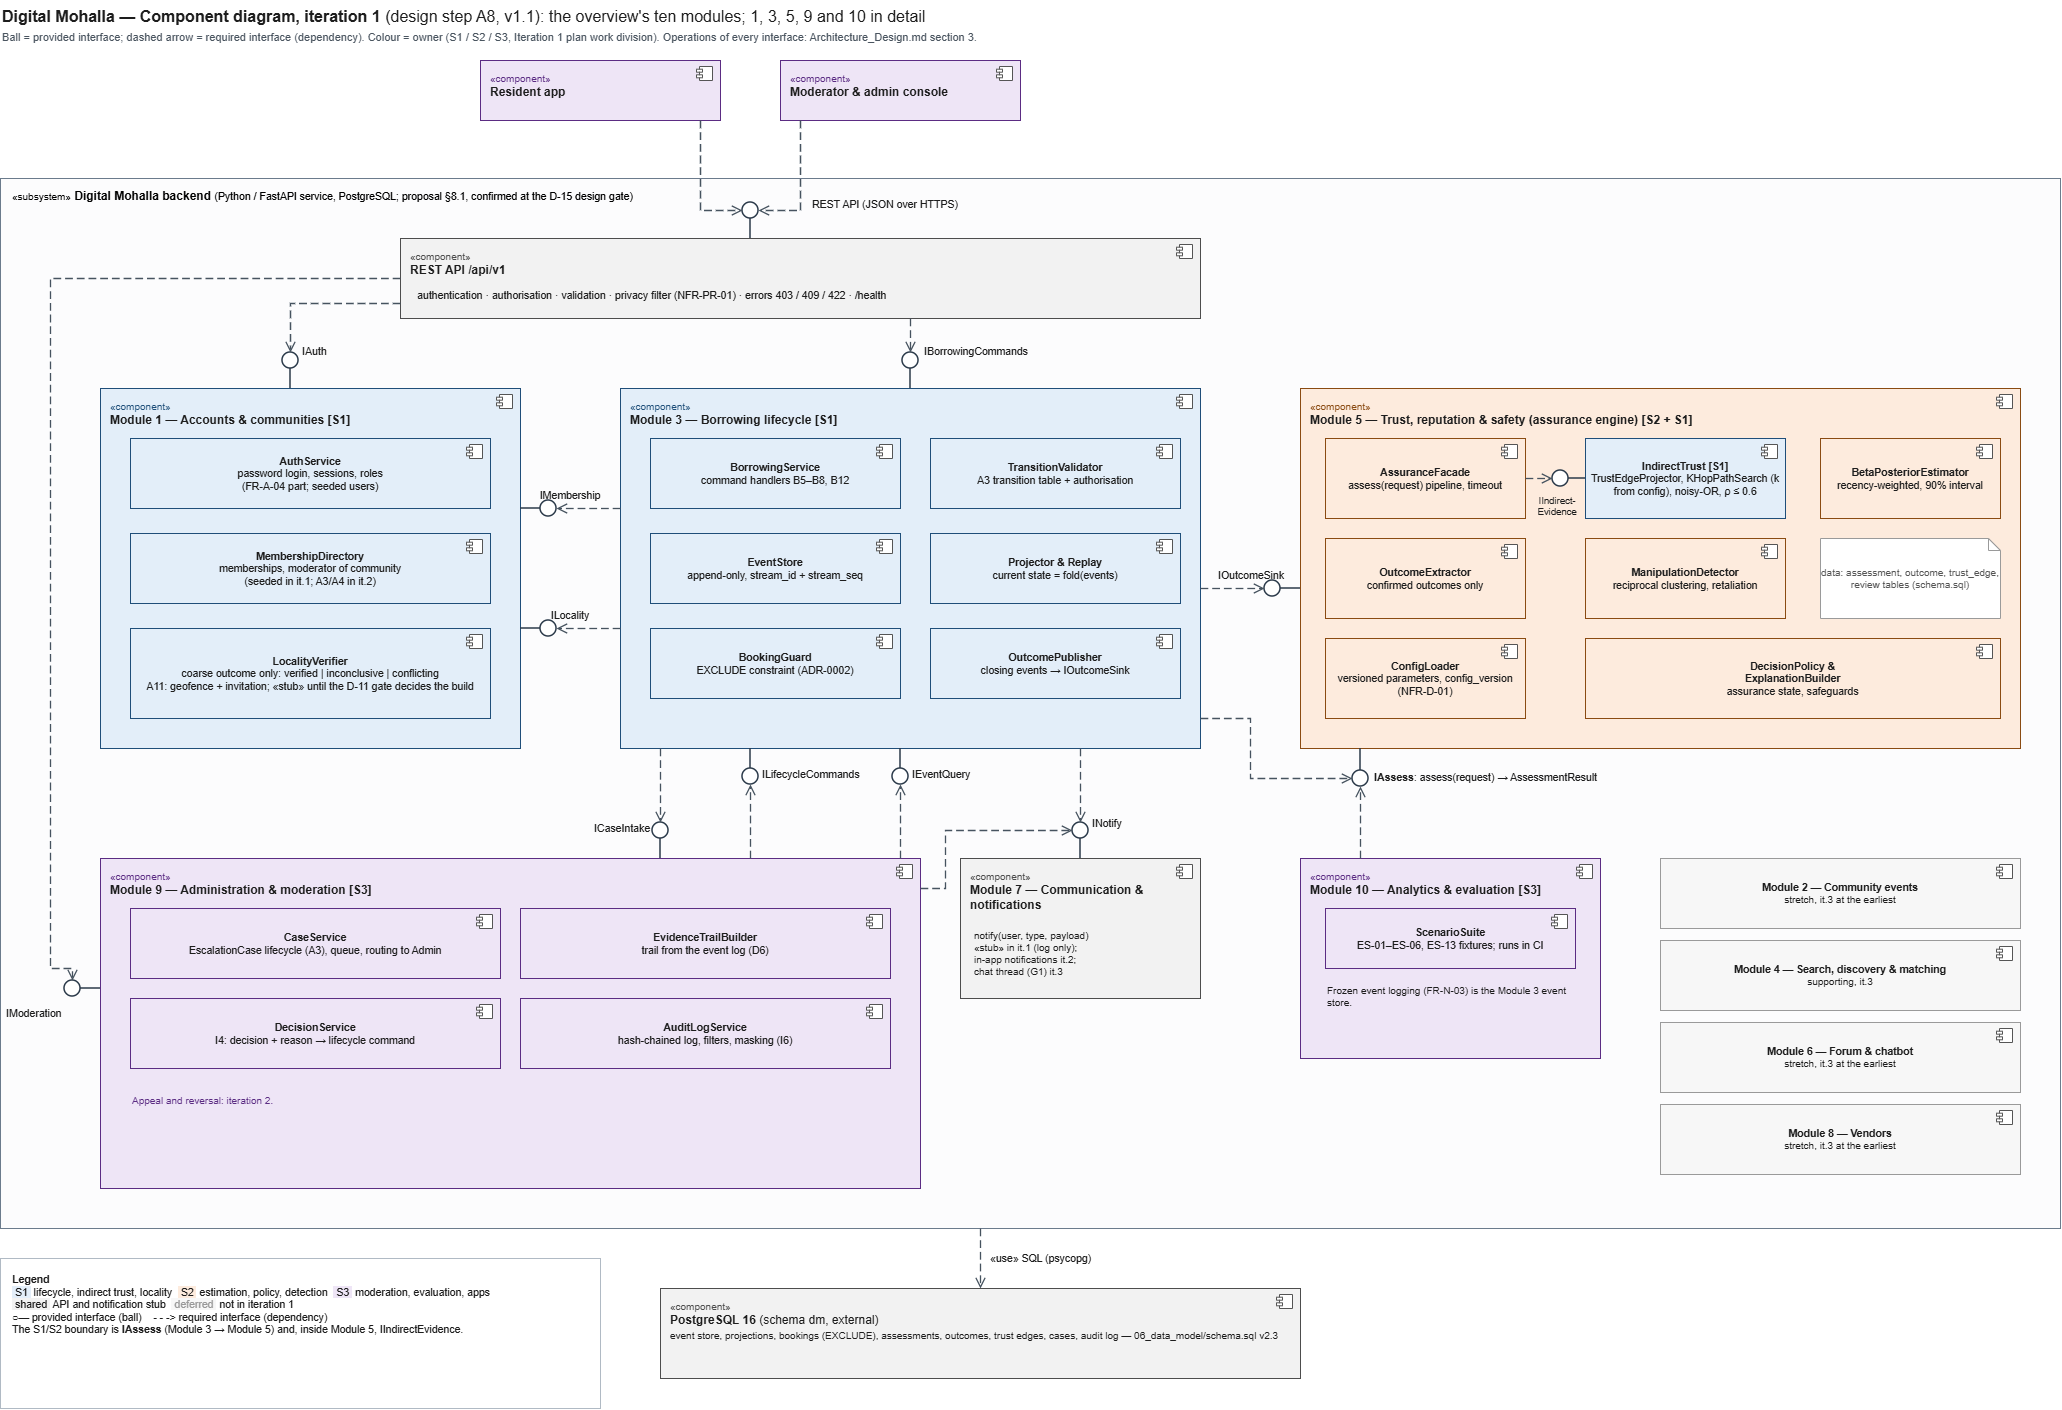
\includegraphics[width=0.85\textwidth]{../../design/03_architecture/component_diagram.drawio.png}
\caption{Component Architecture Diagram showing subsystem boundaries and interfaces}
\label{fig:component_diagram}
\end{figure}

\begin{figure}[htbp]
\centering
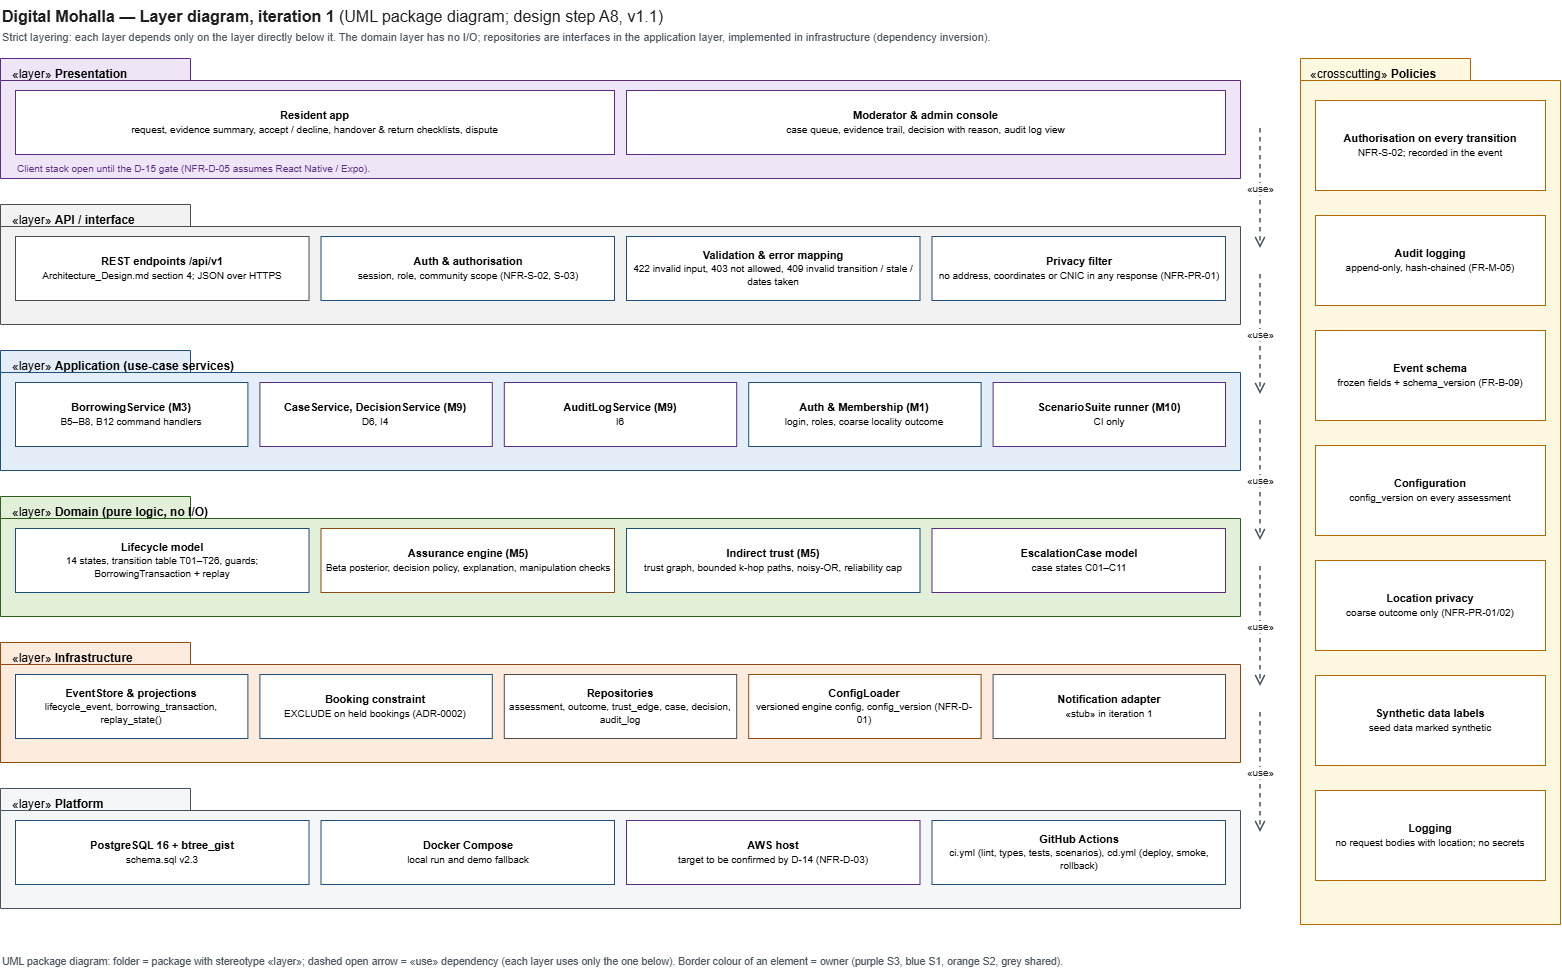
\includegraphics[width=0.85\textwidth]{../../design/03_architecture/layer_diagram.drawio.png}
\caption{Clean Architecture 5-Layer Stack and Dependency Rule}
\label{fig:layer_diagram}
\end{figure}

\begin{figure}[htbp]
\centering
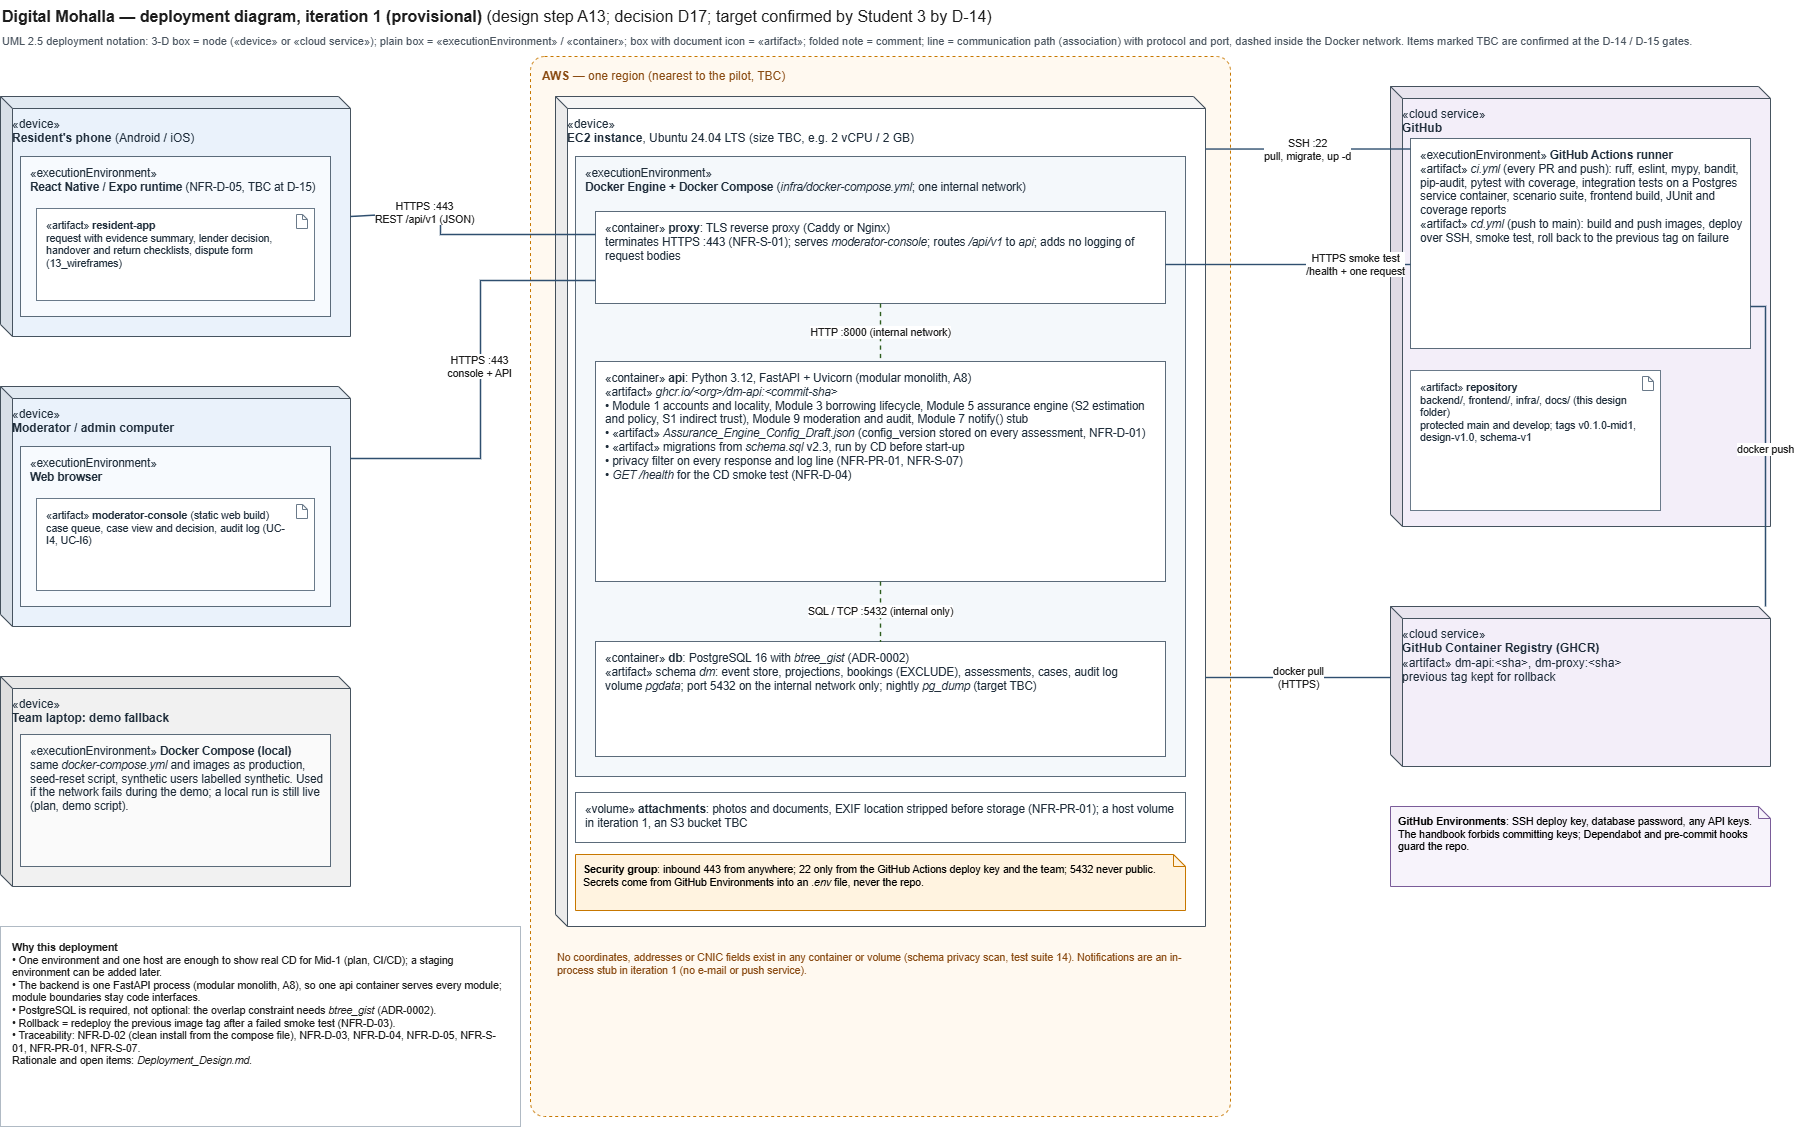
\includegraphics[width=0.85\textwidth]{../../design/04_deployment/deployment_diagram.drawio.png}
\caption{Physical Deployment Topology across Azure Container Apps and Cloud Services}
\label{fig:deployment_diagram}
\end{figure}

\section{Domain and Data Persistence Design}
The relational database schema is managed via Alembic migration \texttt{0001\_schema\_v2\_3.py}. The core entities comprise:
\begin{itemize}
    \item \texttt{users} and \texttt{communities}: User accounts, argon2 password hashes, and coarse locality zone associations.
    \item \texttt{items}: Catalog listings, category classification, replacement value tier, and owner references.
    \item \texttt{lifecycle\_events}: The immutable, append-only event log containing stream UUID, sequence number, event type, cryptographic SHA-256 hash, and JSON payload.
    \item \texttt{borrowing\_requests}: The transactional read model maintaining current status, scheduled dates, and lender/borrower IDs.
    \item \texttt{trust\_edges}: Directed graph edges representing verified direct interaction outcomes between community members.
\end{itemize}

\begin{figure}[htbp]
\centering
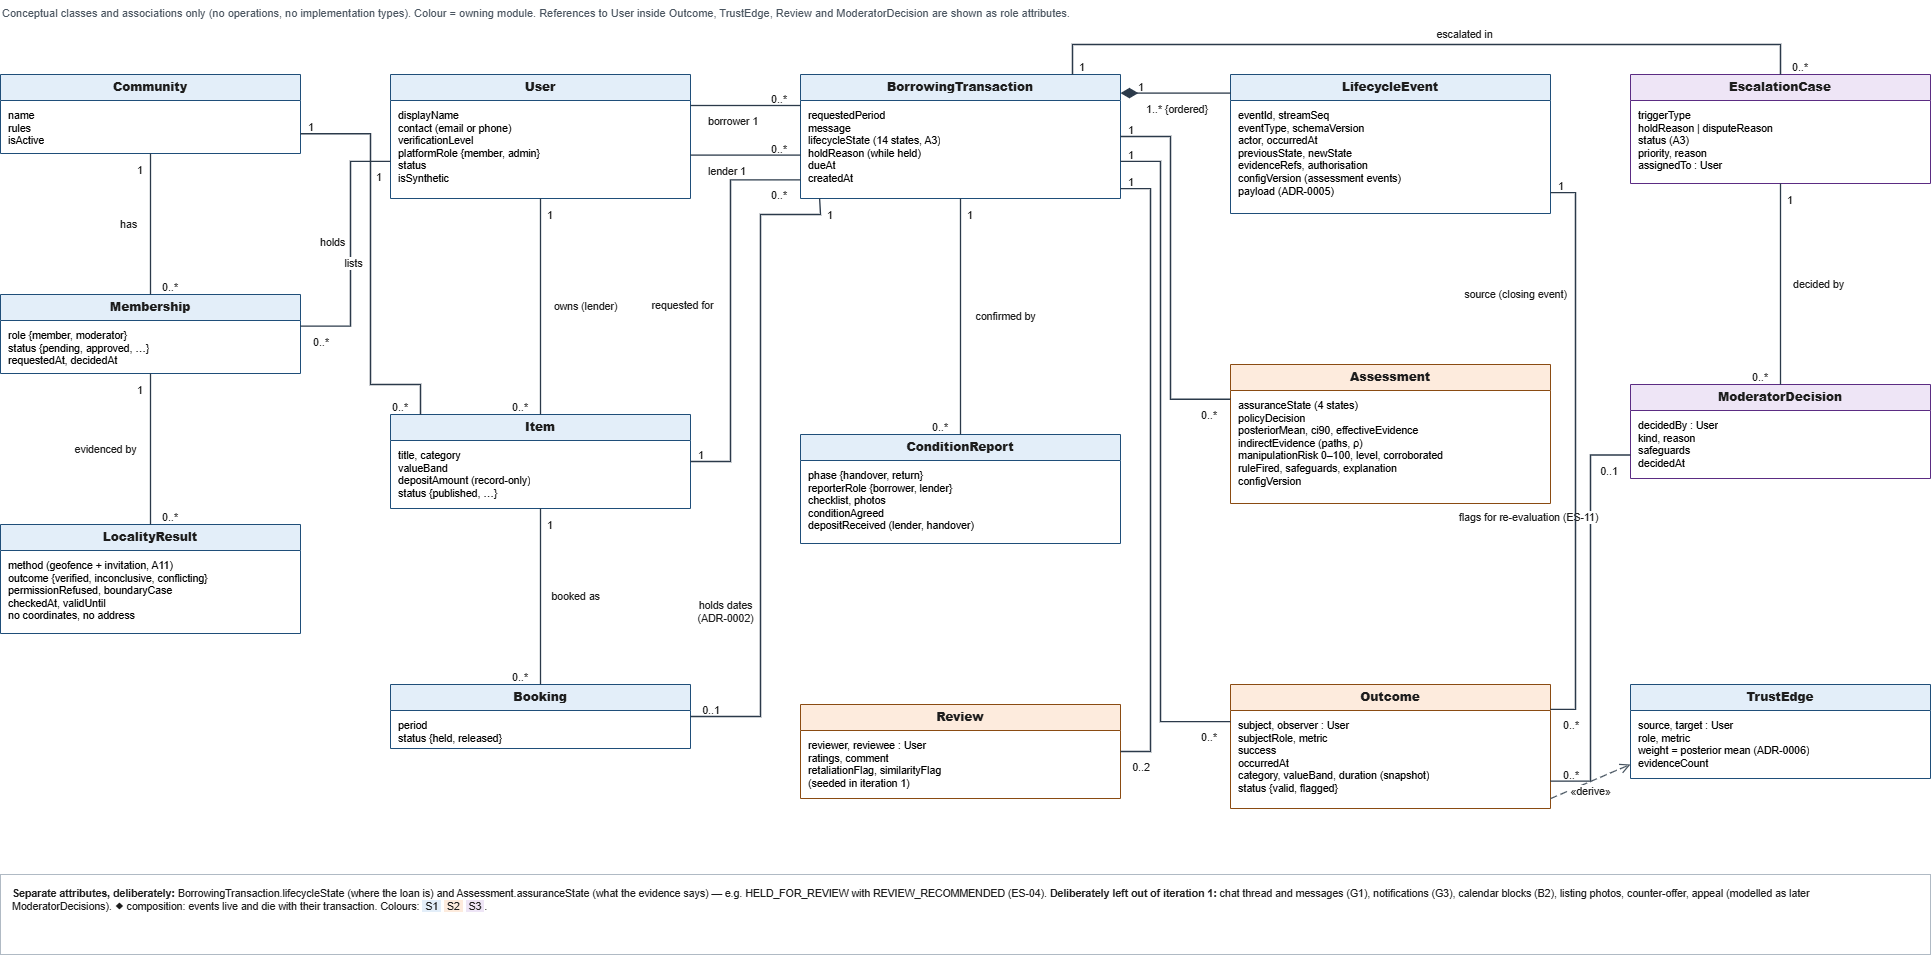
\includegraphics[width=0.85\textwidth]{../../design/05_class_model/domain_model.drawio.png}
\caption{Domain Model representing Aggregates, Value Objects, and Domain Events}
\label{fig:domain_model}
\end{figure}

\begin{figure}[htbp]
\centering
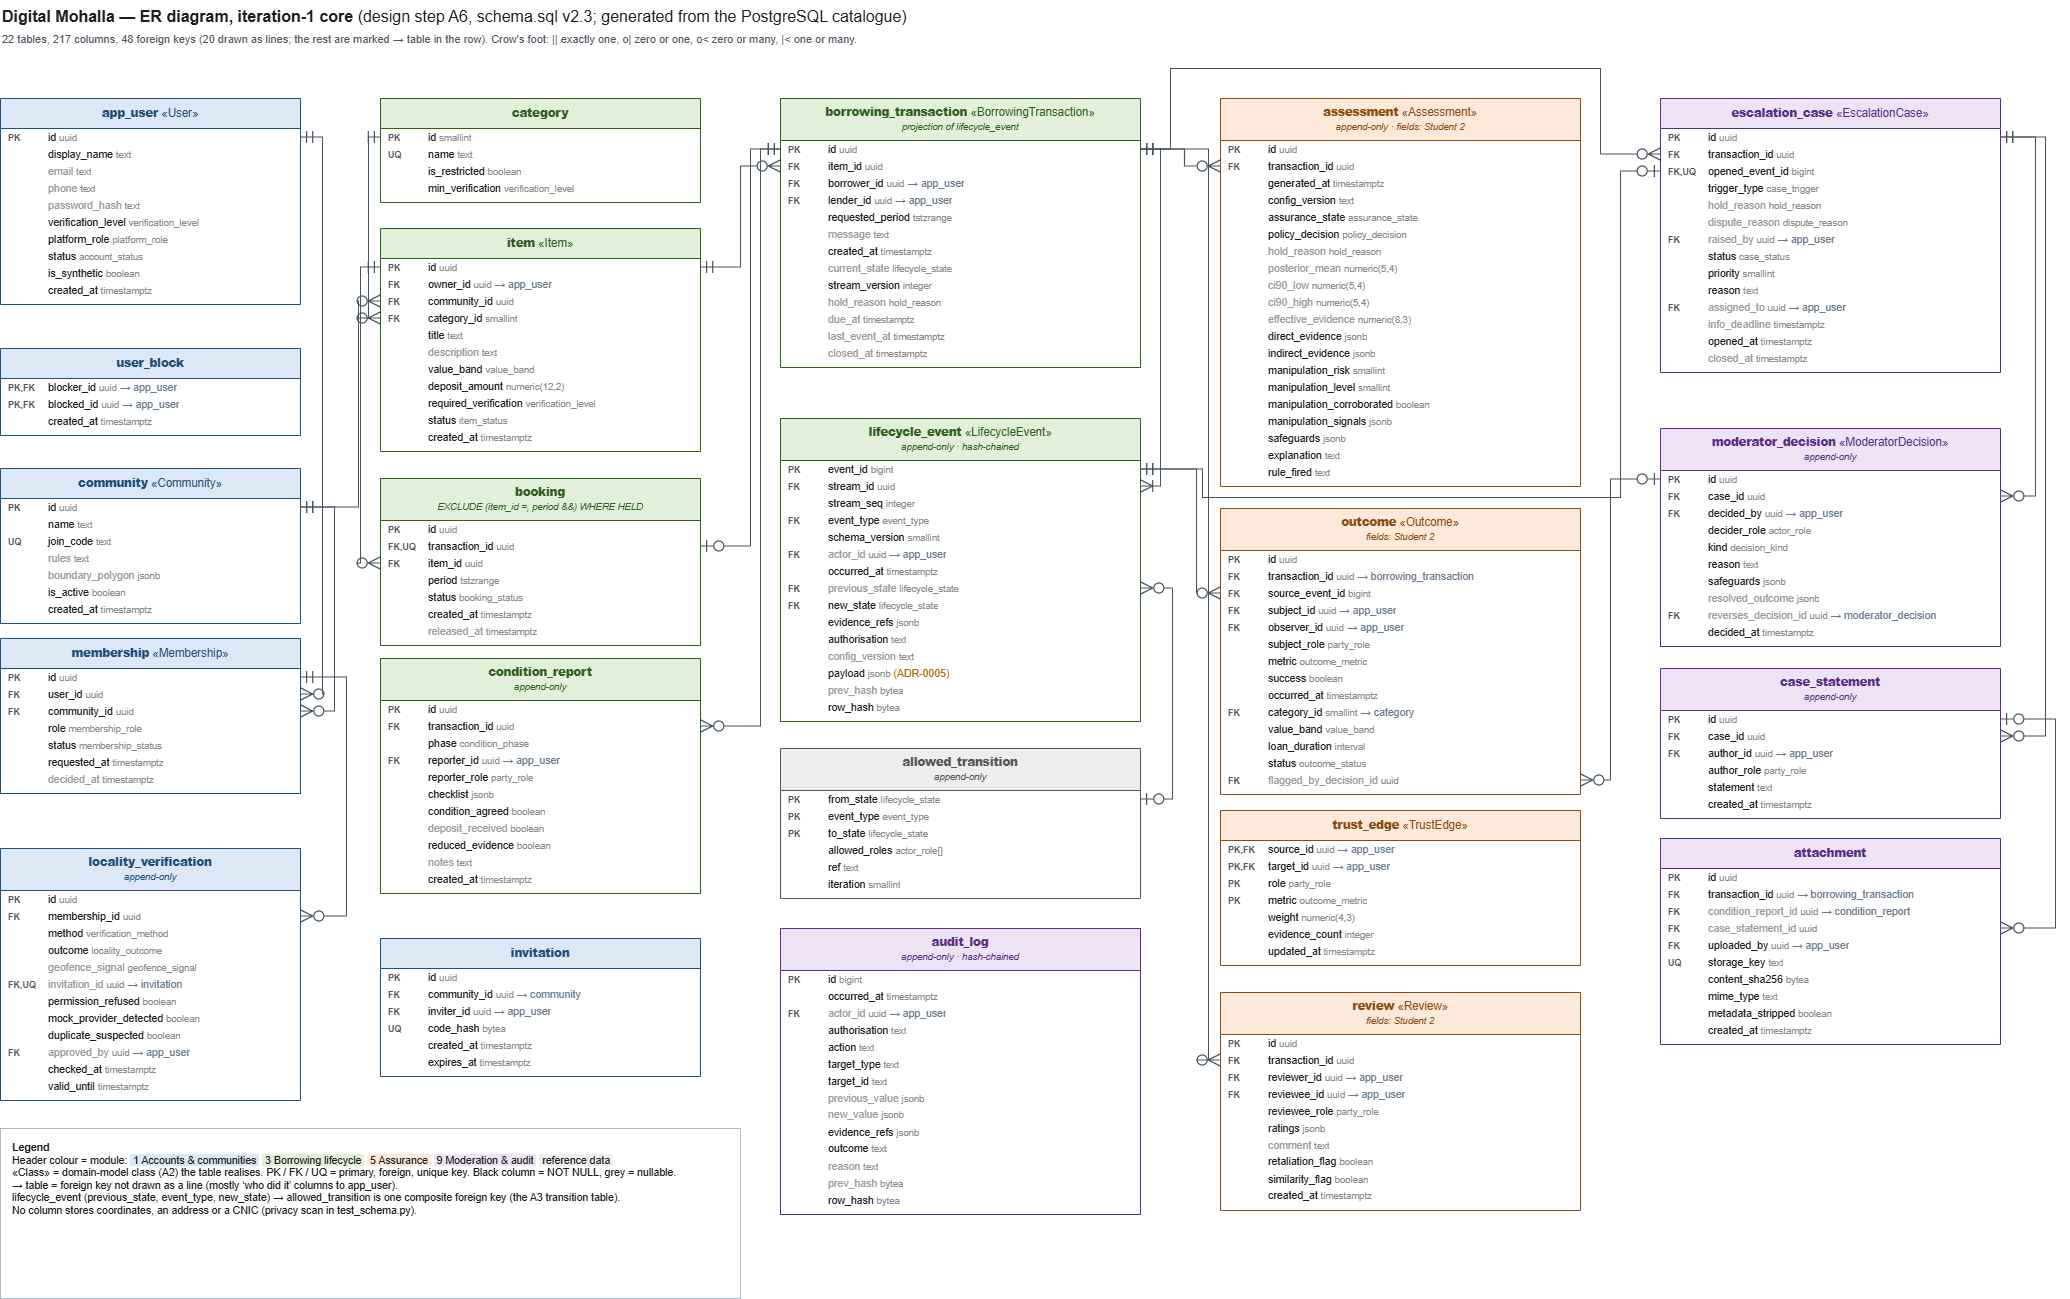
\includegraphics[width=0.85\textwidth]{../../design/06_data_model/er_diagram.drawio.png}
\caption{Entity Relationship Diagram (ERD v2.3 Specification)}
\label{fig:erd_diagram}
\end{figure}

\section{Behavioral and Dynamic State Design}
The borrowing lifecycle is governed by a strict finite state machine:
\begin{equation}
    \text{REQUEST\_CREATED} \rightarrow \text{LOCALITY\_CHECKED} \rightarrow \text{ASSESSED} \rightarrow \text{ACCEPTED} \rightarrow \text{ACTIVE} \rightarrow \text{RETURN\_INITIATED} \rightarrow \text{RETURNED} \rightarrow \text{COMPLETED}
\end{equation}
Alternative branching paths handle rejections, cancellations, timeouts, and review holds. All valid transitions and all 294 invalid transition combinations are explicitly tested.

\begin{figure}[htbp]
\centering
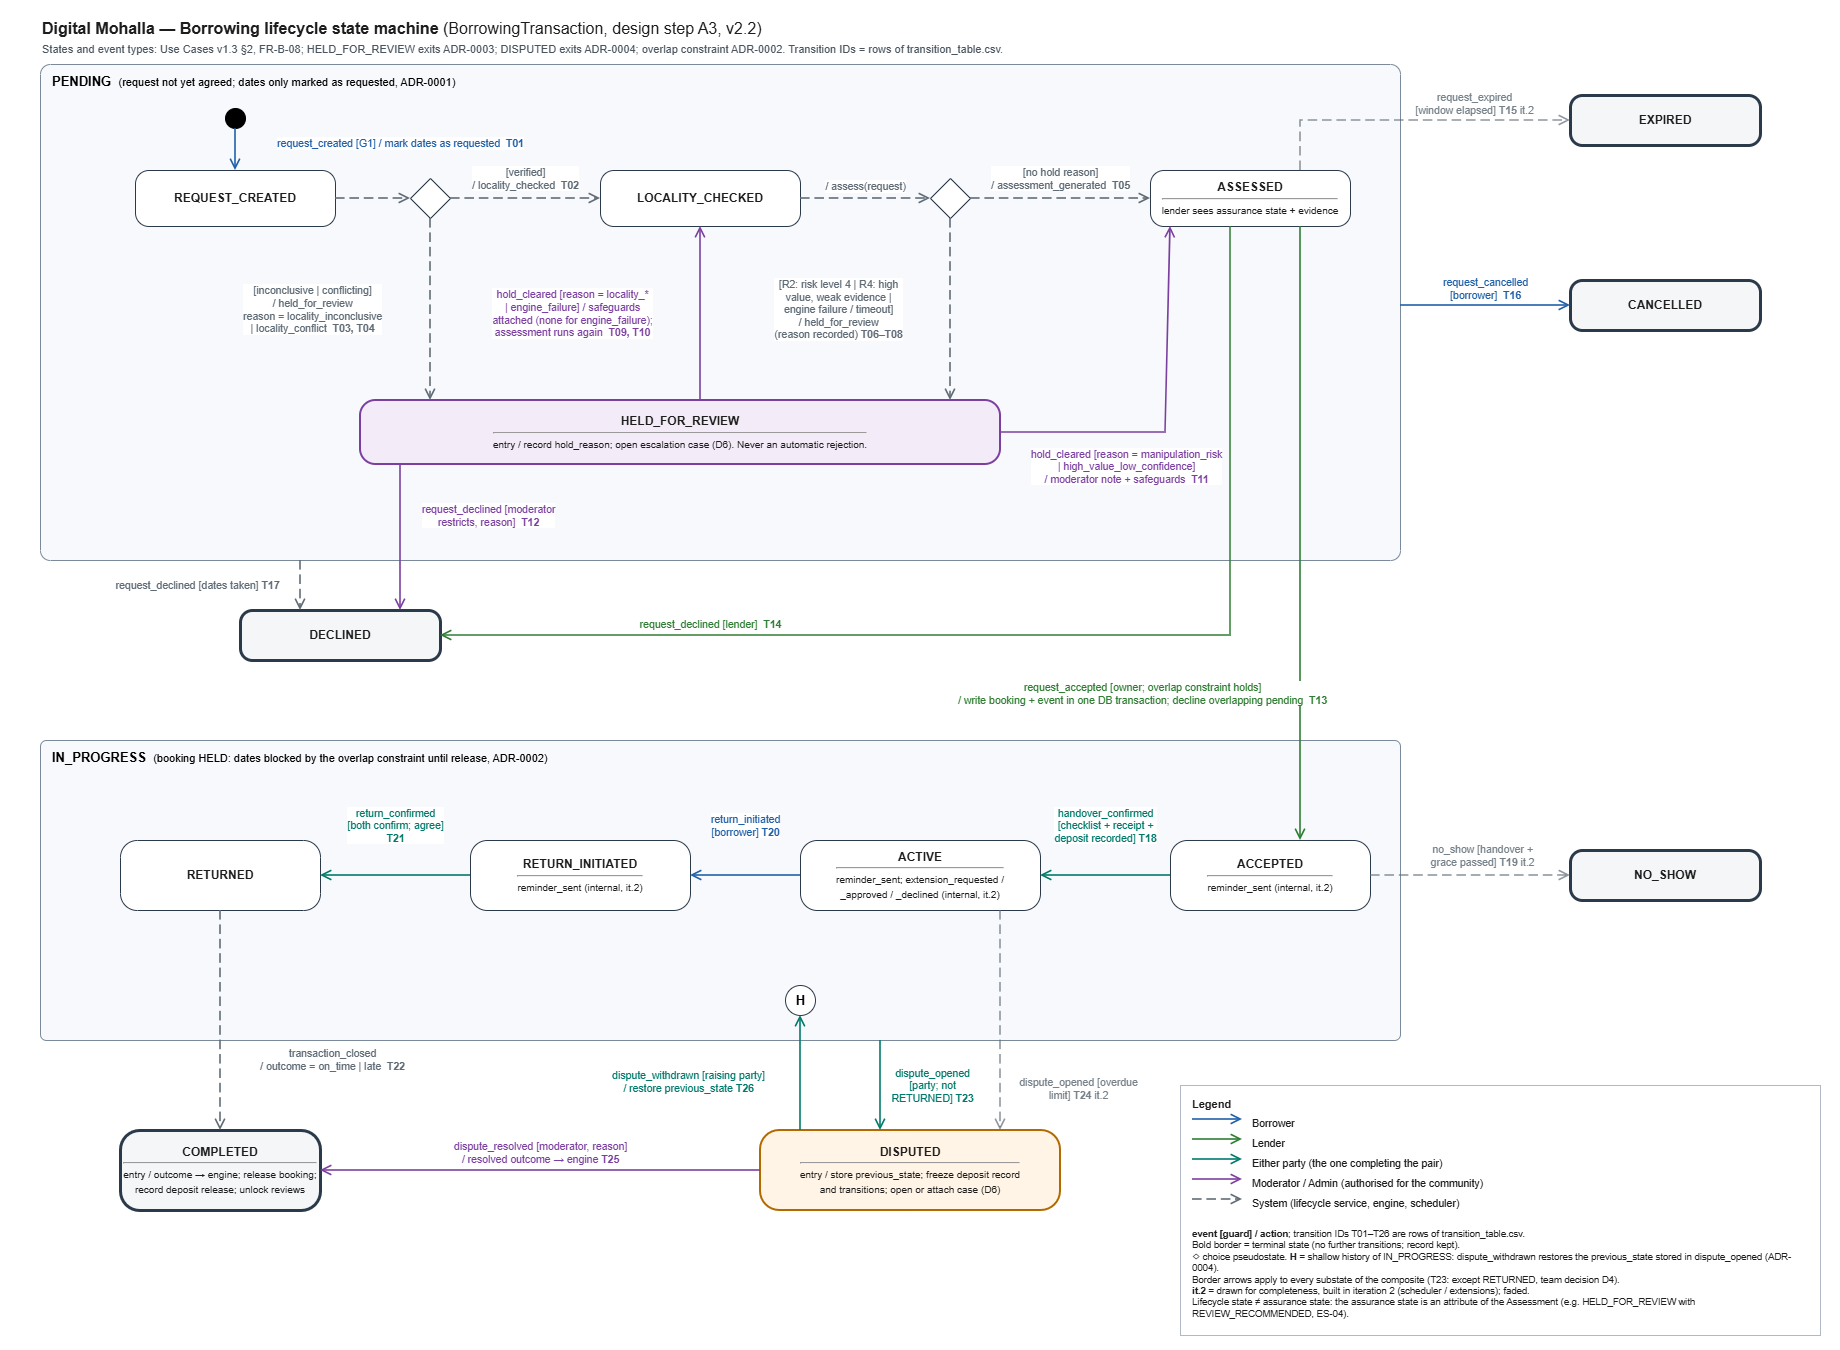
\includegraphics[width=0.85\textwidth]{../../design/07_state_machines/borrowing_lifecycle_state_machine.drawio.png}
\caption{Borrowing Lifecycle State Machine and Verified Transition Flows}
\label{fig:state_machine}
\end{figure}

\begin{figure}[htbp]
\centering
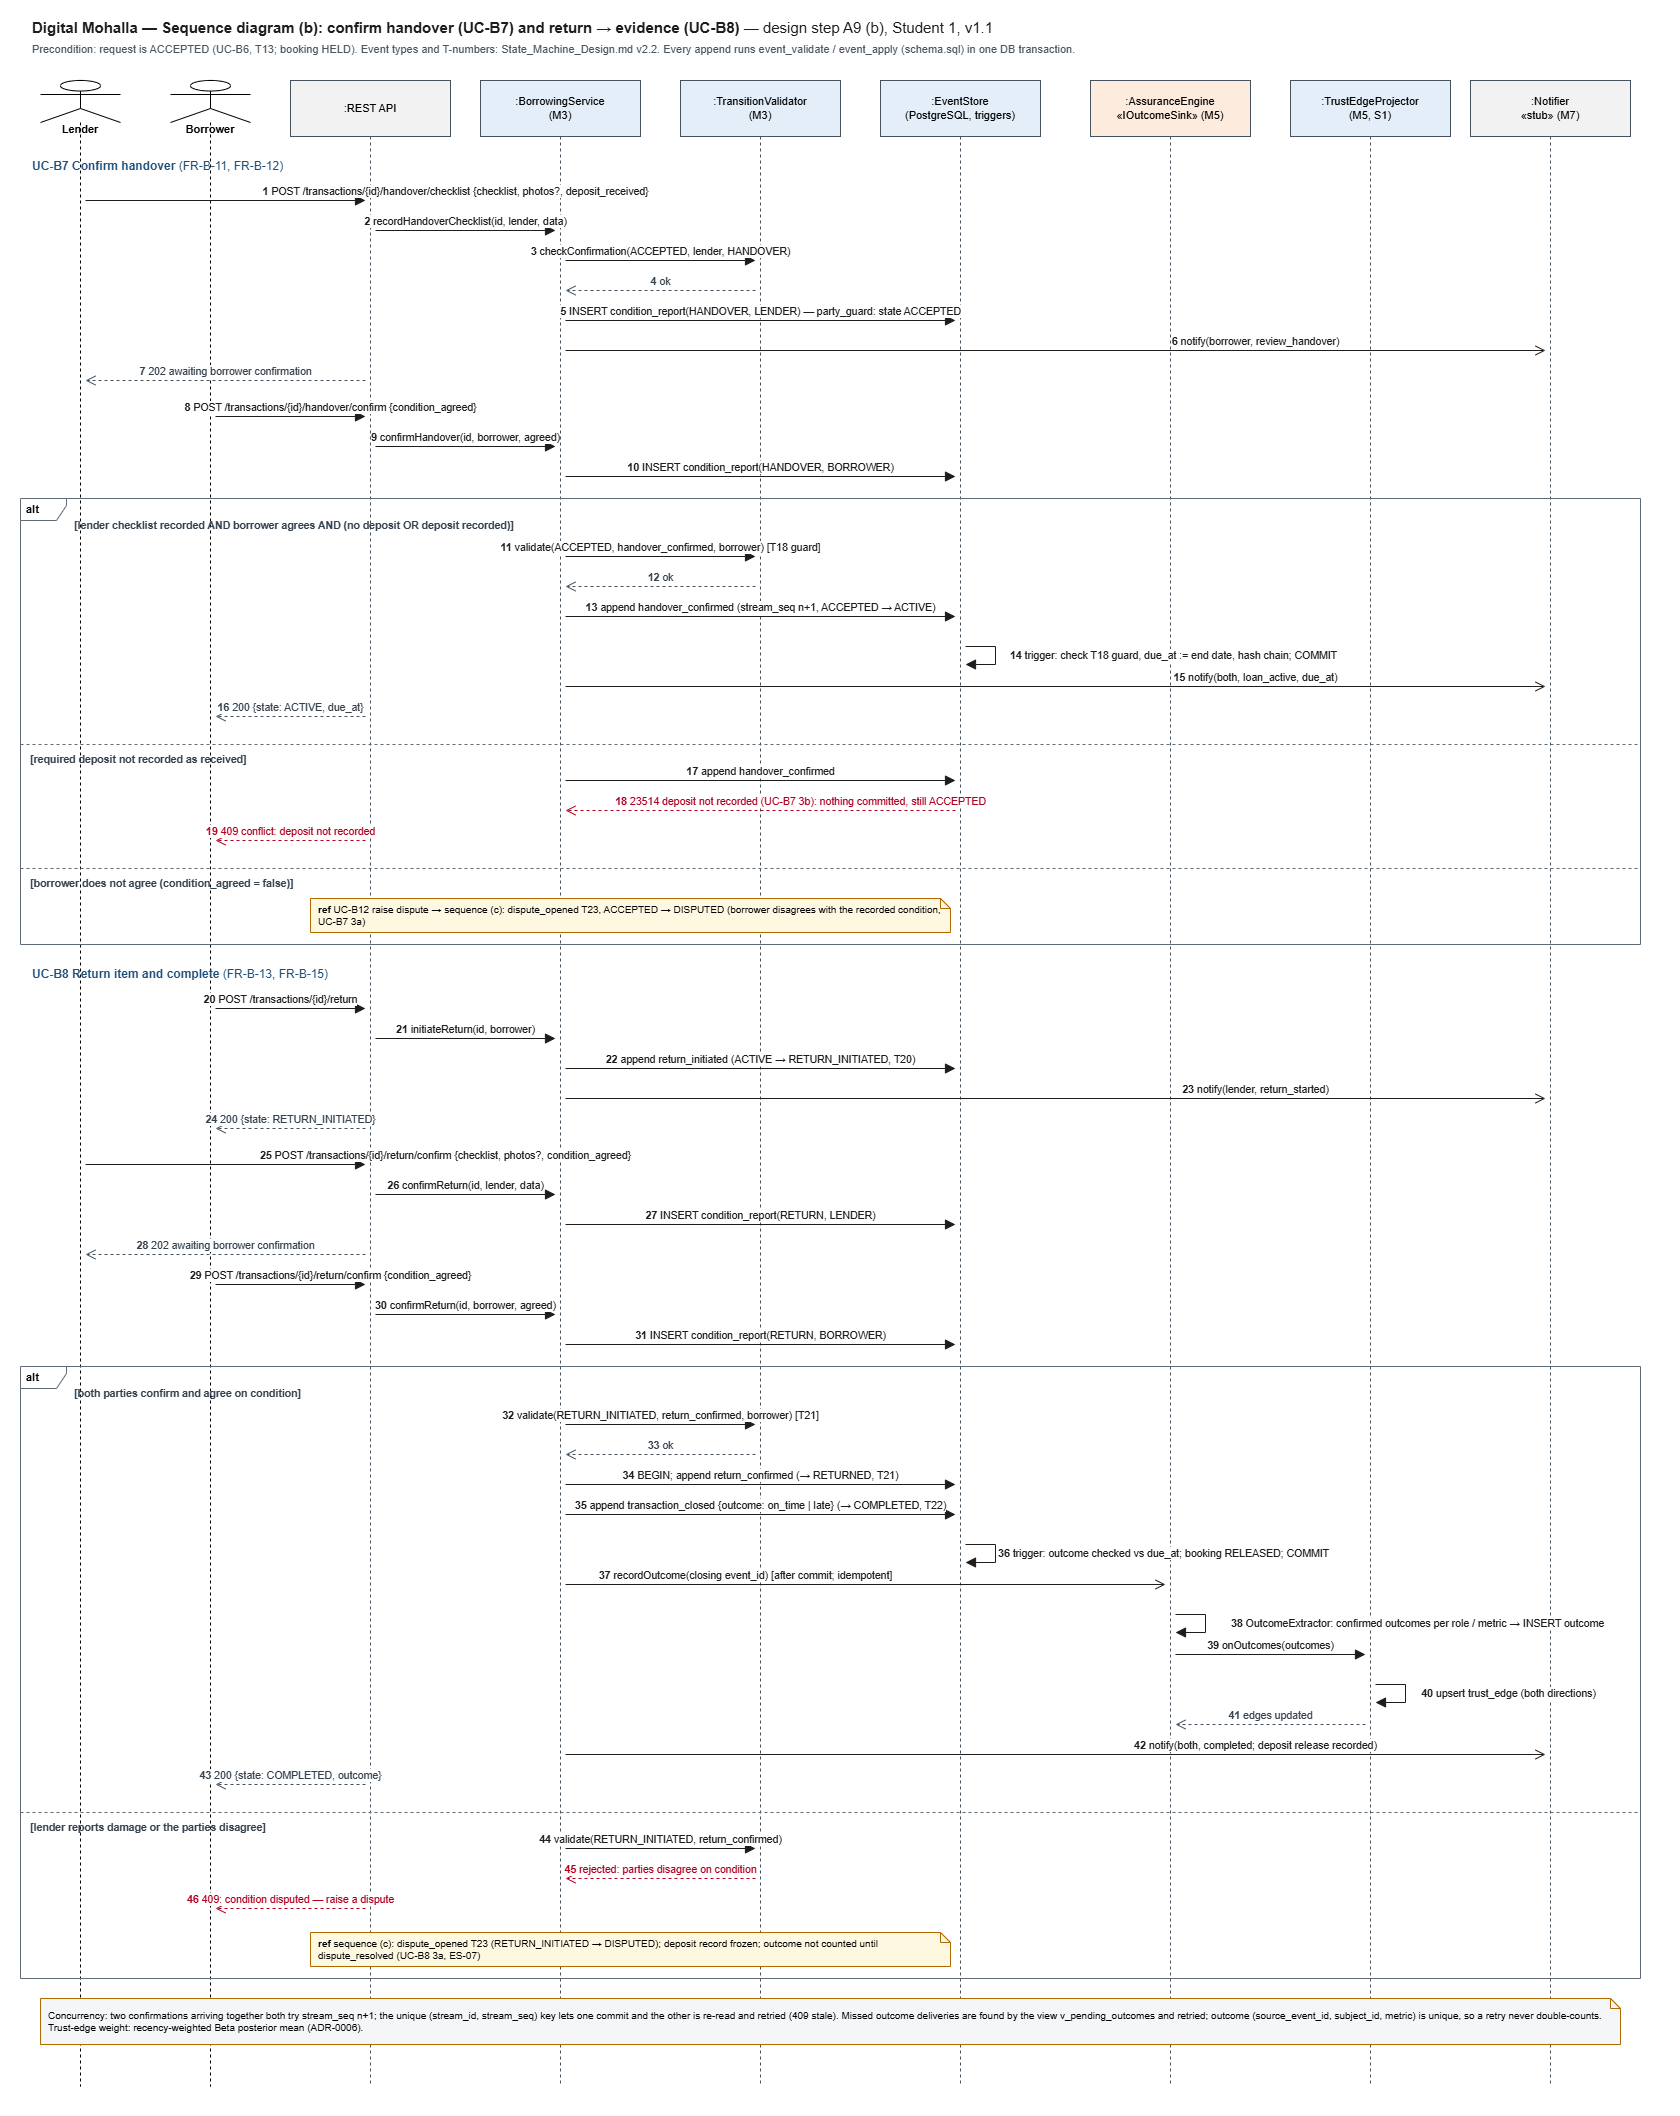
\includegraphics[width=0.85\textwidth]{../../design/08_sequence_diagrams/sequence_b_handover_return.drawio.png}
\caption{Sequence Diagram: Handover Verification and Dual-Party Return Confirmation}
\label{fig:seq_handover_return}
\end{figure}

\begin{figure}[htbp]
\centering
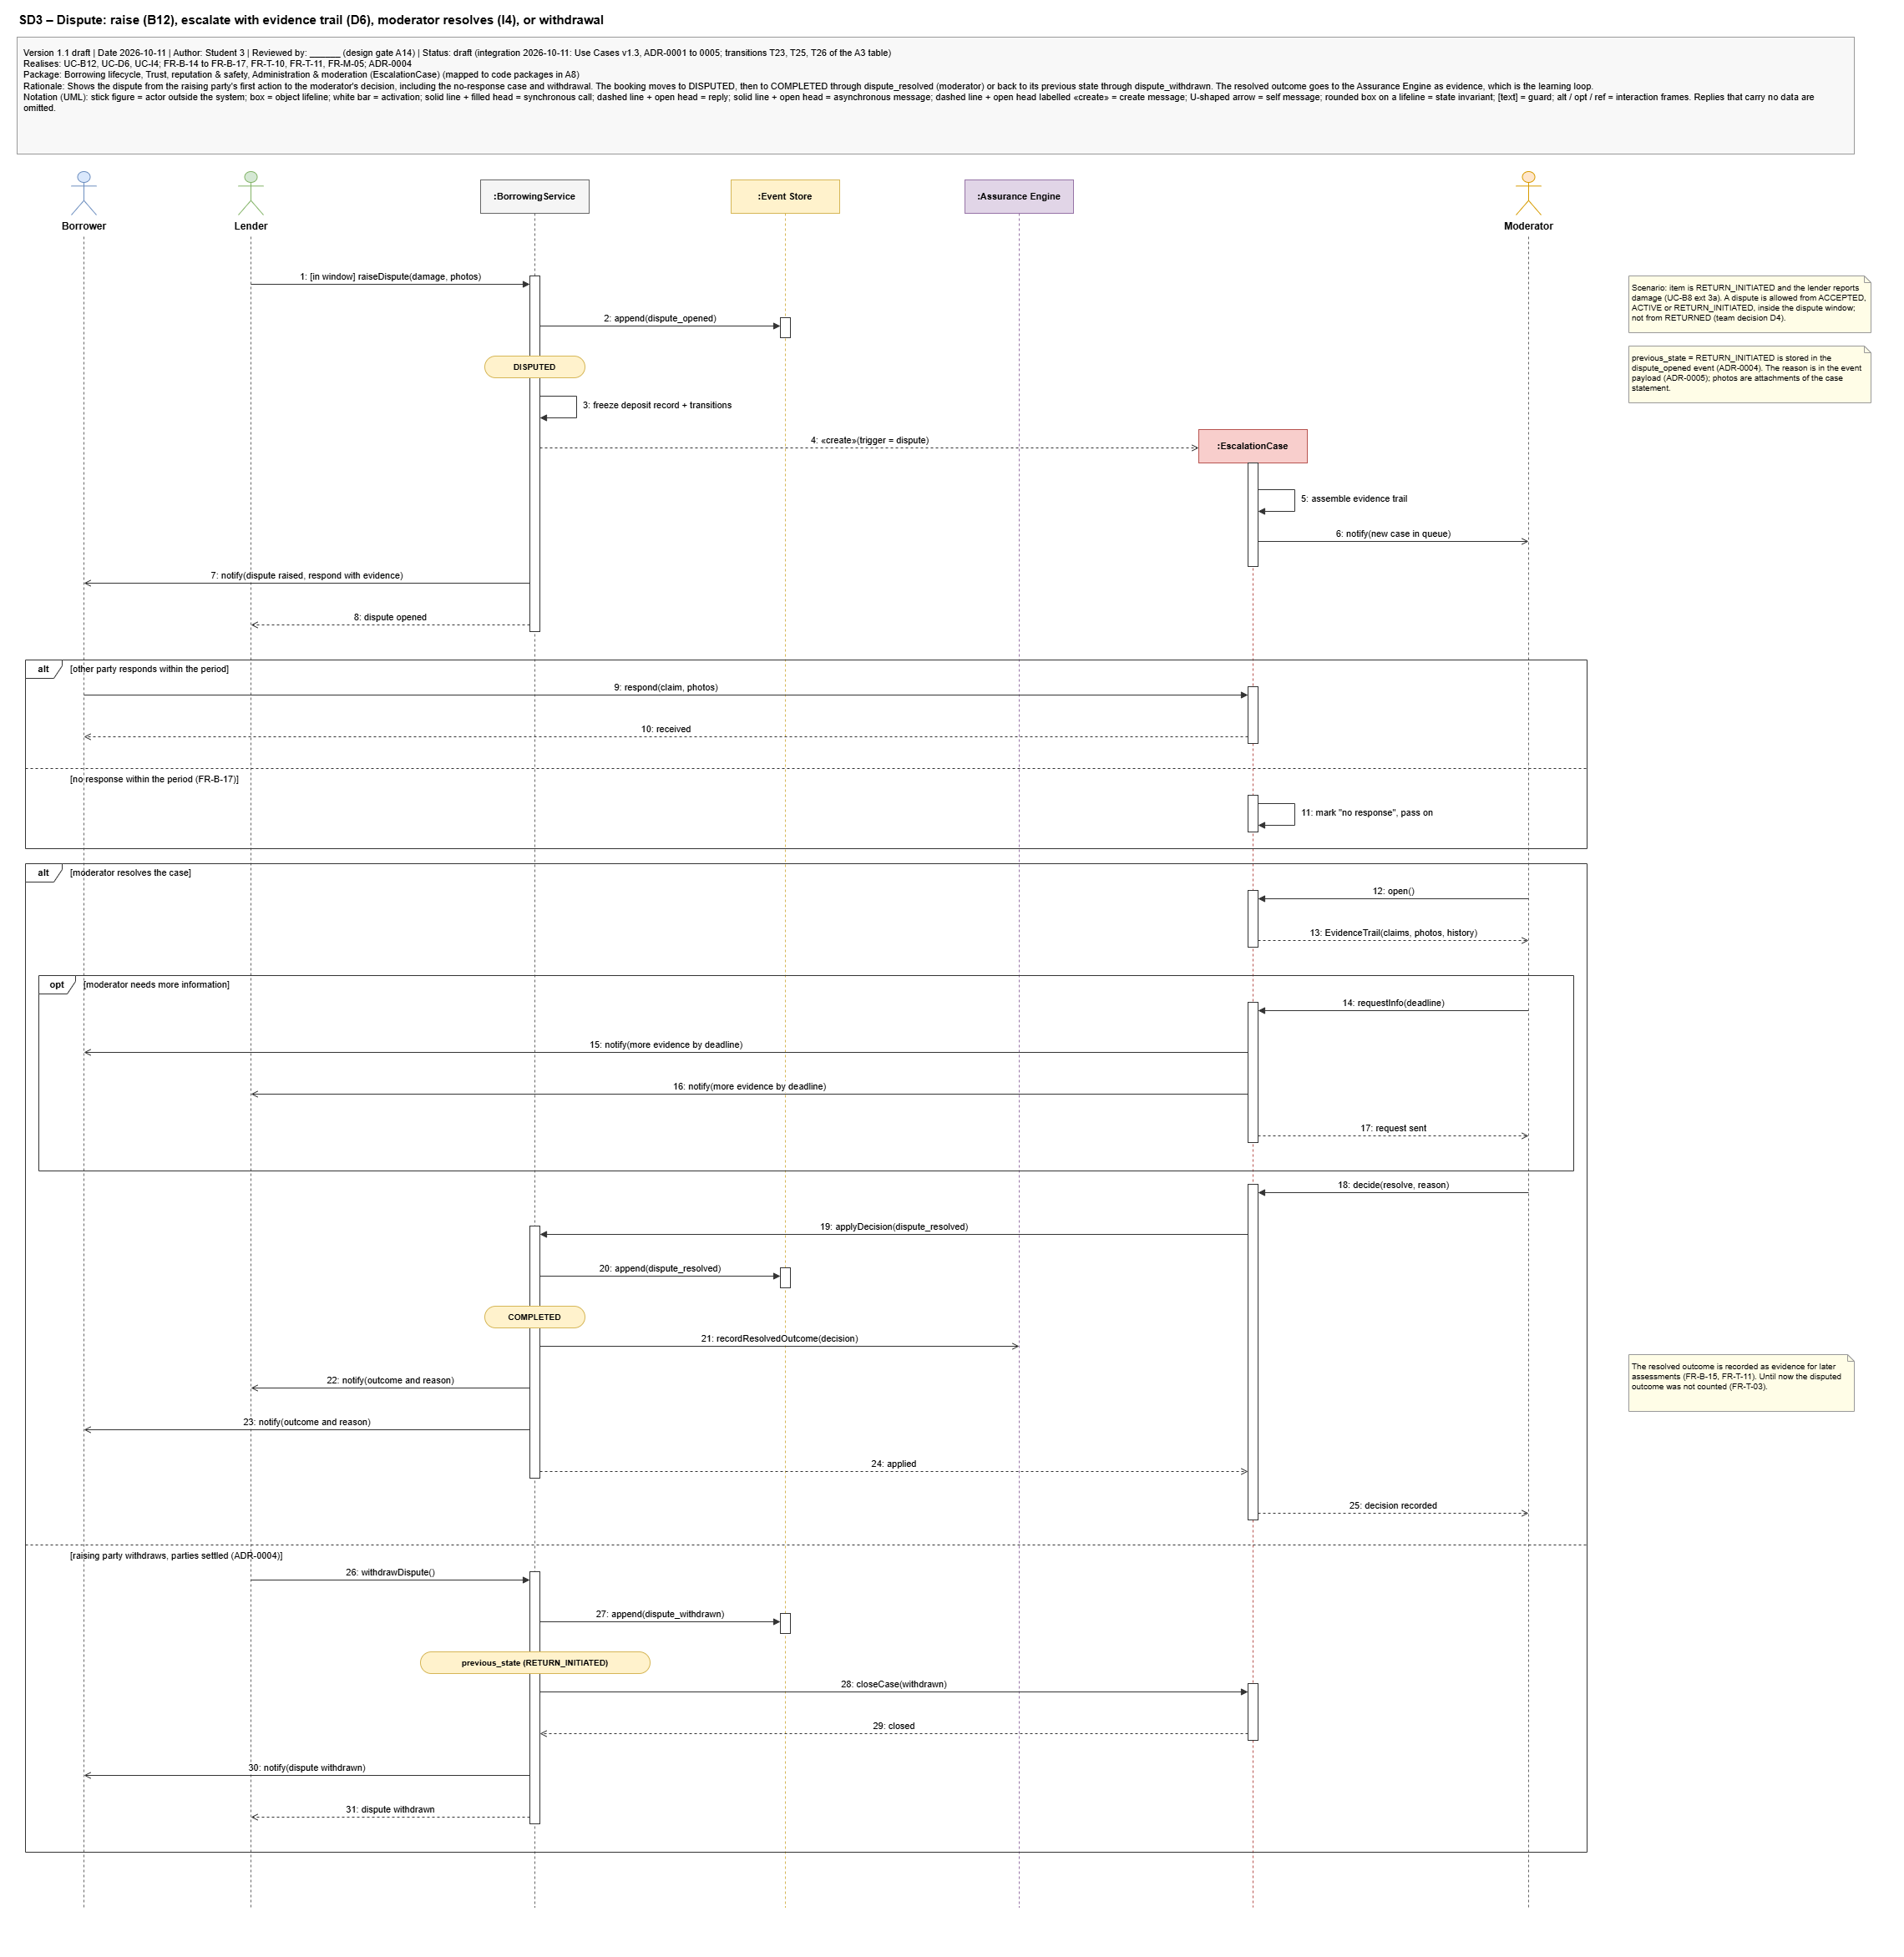
\includegraphics[width=0.85\textwidth]{../../design/08_sequence_diagrams/sequence_c_dispute.drawio.png}
\caption{Sequence Diagram: Dispute Filing, Moderator Escalation, and Evidence Packaging}
\label{fig:seq_dispute}
\end{figure}

\begin{figure}[htbp]
\centering
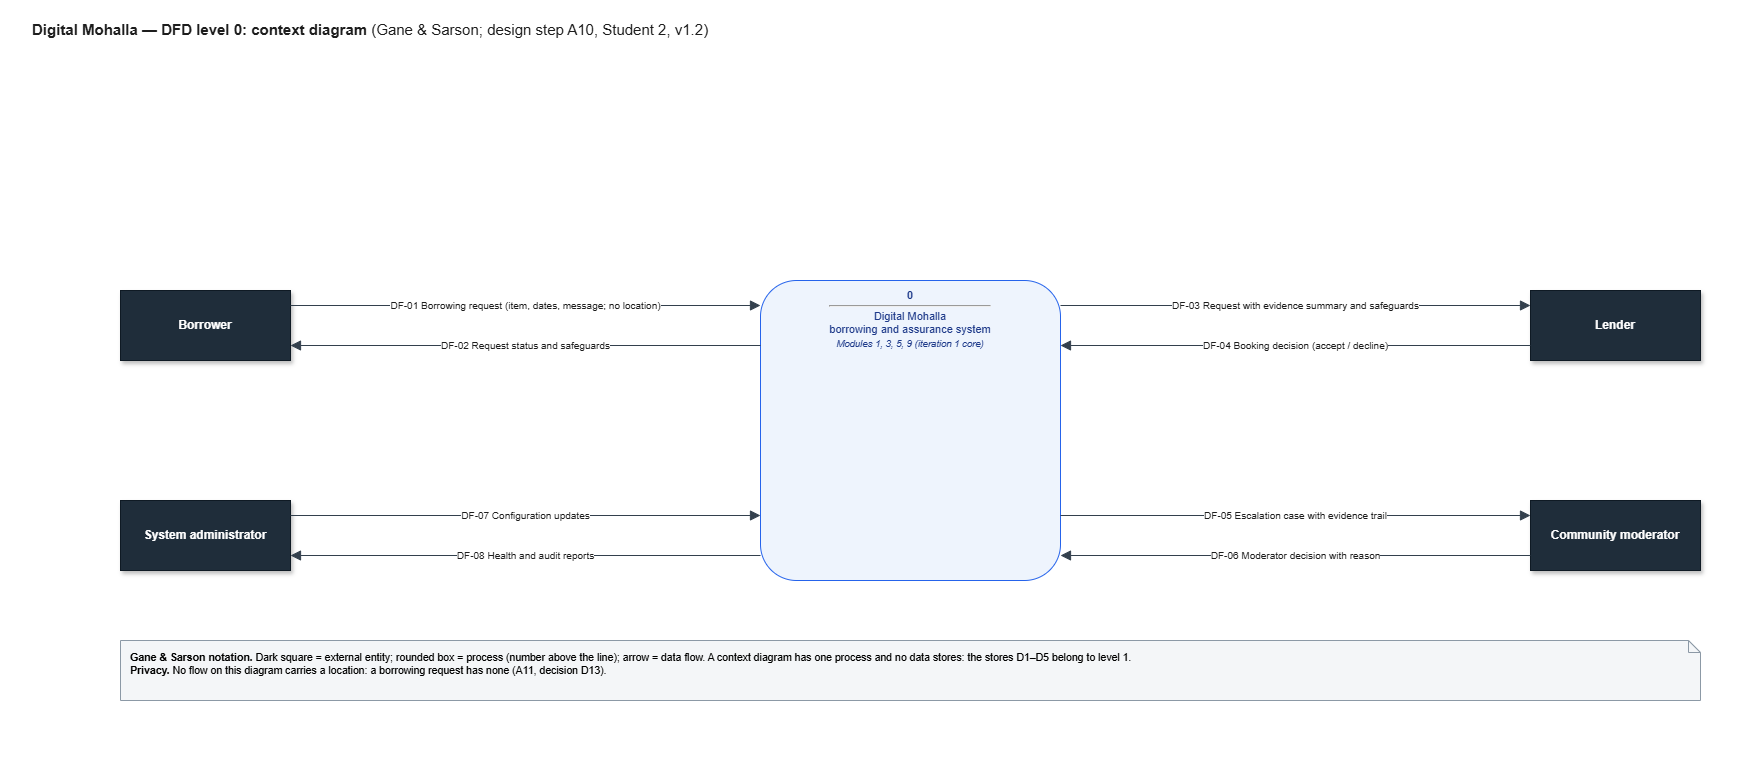
\includegraphics[width=0.85\textwidth]{../../design/10_dfd/dfd_assurance_pipeline_level0_level1-DFD level 0 (context).drawio.png}
\caption{Data Flow Diagram: Assurance Pipeline Context (Level 0)}
\label{fig:dfd_context}
\end{figure}

\section{Design Artefacts and Diagram Registry}
Table \ref{tab:design_artefacts} catalogues the formal design artefacts developed during Iteration 1.

\begin{table}[htbp]
\centering
\caption{Design Artefacts Register (UML 2.5 Baseline)}
\label{tab:design_artefacts}
\small
\begin{tabularx}{\textwidth}{l p{6.5cm} l l}
\toprule
\textbf{Artefact ID} & \textbf{Diagram / Model Name} & \textbf{File Location} & \textbf{Status} \\
\midrule
ART-01 & Component Architecture Diagram & \texttt{docs/design/03\_architecture/component\_diagram.drawio} & Complete \\
ART-02 & Layer Architecture Diagram & \texttt{docs/design/03\_architecture/layer\_diagram.drawio} & Complete \\
ART-03 & Deployment Architecture Diagram & \texttt{docs/design/04\_deployment/deployment\_diagram.drawio} & Complete \\
ART-04 & Domain Class Model (S1, S2, S3) & \texttt{docs/design/05\_class\_model/} & Complete \\
ART-05 & Entity Relationship Diagram (ERD v2.3) & \texttt{docs/design/06\_data\_model/er\_diagram.drawio} & Complete \\
ART-06 & Lifecycle State Machine & \texttt{docs/design/07\_state\_machines/} & Complete \\
ART-07 & Sequence Diagram: Request to Assessment & \texttt{docs/design/08\_sequence\_diagrams/sequence\_a.drawio} & Complete \\
ART-08 & Sequence Diagram: Handover \& Return & \texttt{docs/design/08\_sequence\_diagrams/sequence\_b.drawio} & Complete \\
ART-09 & Assurance Pipeline DFD (L0 \& L1) & \texttt{docs/design/10\_dfd/dfd\_assurance\_pipeline.drawio} & Complete \\
ART-10 & Wireframes Suite (W1--W8) & \texttt{docs/design/13\_wireframes/} & Complete \\
\bottomrule
\end{tabularx}
\end{table}
\textit{Note on Diagrams:} In accordance with FAST-NUCES submission standards, vector/raster versions of all \texttt{.drawio} XML files can be exported to PNG format (300 DPI) and stored directly in \texttt{figures/} for automatic inclusion in the compiled thesis.
